\documentclass[a4paper,12pt]{article} \usepackage[swedish]{babel}
\usepackage[utf8]{inputenc} \usepackage{amsmath, amsthm, amssymb, tikz}
\usetikzlibrary{decorations.pathreplacing}
\usepackage[a4paper,includeheadfoot,margin=2.54cm]{geometry}
\usepackage[left]{lineno}

\newcommand*\patchAmsMathEnvironmentForLineno[1]{% \expandafter\let\csname
    old#1\expandafter\endcsname\csname #1\endcsname \expandafter\let\csname
    oldend#1\expandafter\endcsname\csname end#1\endcsname
    \renewenvironment{#1}% {\linenomath\csname old#1\endcsname}% {\csname
    oldend#1\endcsname\endlinenomath}}%
    \newcommand*\patchBothAmsMathEnvironmentsForLineno[1]{%
        \patchAmsMathEnvironmentForLineno{#1}%
        \patchAmsMathEnvironmentForLineno{#1*}}% \AtBeginDocument{%
        \patchBothAmsMathEnvironmentsForLineno{equation}%
        \patchBothAmsMathEnvironmentsForLineno{align}%
        \patchBothAmsMathEnvironmentsForLineno{flalign}%
        \patchBothAmsMathEnvironmentsForLineno{alignat}%
        \patchBothAmsMathEnvironmentsForLineno{gather}%
        \patchBothAmsMathEnvironmentsForLineno{multline}% }

        \renewcommand\linenumberfont{\normalfont\bfseries\small}

        \title{Jämförelse av algoritmer}
        %
        \author{Zacharias Brohn\thanks{email:
        \texttt{zacbro-8@student.ltu.se}}\\  ~ \\ Luleå tekniska universitet \\
        971 87 Luleå, Sverige}
        %
        \date{\today}
        %
        \begin{document} \linenumbers % ger radnumrering \maketitle
        %
        \begin{abstract} Denna rapport kommer att förklara och jämföra olika
            algoritmer för att undersöka hur de skiljer sig i både utförning
            och prestanda. Algoritmerna i fråga används för att den största
            summan av en sekvens av nummer i en array. Den första algoritmen är
            en kubisk algoritm som har en komplexitet av $O\left(N^3\right)$,
            och sedan har vi två kvadratiska algoritmer som har en komplexitet
        av $O\left(N^2\right)$. \end{abstract}
        %
        \section{Introduktion} \label{sec:introduktion} Big-Oh, även kallat
        komplexitet, är namnet på ett uttryck som används för att beskriva
        hur många steg en algoritm tar för att nå ett svar i det
        \textbf{värsta fallet}. Låt oss illustrera detta med hjälp av ett
        välkänt exempel som också gör det lättare att förstå problemet vi
        ska undersöka i rapporten: \subsection*{Telefonboken} Om vi
        beskriver $N$ som antalet namn i boken och vi börjar leta överst på
        listan och går sedan stegvis nedför listan tills vi hittar namnet
        vi vill ha betyder att i det \textbf{värsta fallet} är namnet vi
        söker längst ner på listan, så antalet steg som behövs för att
        hitta namnet blir då $N$, lika många namn som finns i listan,
        alltså våran 'algoritm' som hittar namnet vi söker kan beskrivas
        med $O\left(N\right)$.
        %
        \newpage \section{Problembeskrivning: Maximal delfältssumma}
        \label{sec:problembeskrivning} Målet med algoritmerna vi ska
        diskutera är att leta i en array för att hitta en underarray
        (subarray) som har störst summa. Givet en sekvens av reella tal som
        representeras av en array $X$ där $X = [x_1, x_2, \ldots, x_N]$,
        där $N$ är antalet element i arrayen, är målet att hitta den
        maximala summan av ett sammanhängande delfält. Detta innebär att vi
        vill identifiera en del av arrayen, $X[L..U]$, där $1 \leq L \leq U
        \leq N$, för vilken summan \begin{displaymath} S = \sum_{i=L}^{U}
        x_i \end{displaymath} är maximal. Lösningen till problemet är
        enkelt när alla tal $x_i$ är positiva, eftersom då är den maximala
        delfältssumman helt enkelt summan av hela sekvensen:
        \begin{displaymath} \max S = \sum_{i=1}^{N} x_i. \end{displaymath}
            Men utmaningen uppstår när det finns negativa tal i sekvensen.
            I dessa fall måste vi överväga om vi ska inkludera ett negativt
            tal $x_k$, med hopp om att positiva tal bakom och framför,
            $x_{k-1}$ och $x_{k+1}$ summerar den största underarrayen.
            Skulle alla tal i sekvensen $X$ vara negativa, så är den
            största summan av en underarrayen noll: \begin{displaymath}
                \max S = 0 \quad \text{(för alla } x_i < 0\text{)}.
            \end{displaymath} Det enklaste sättet att lösa problemet är att
            iterera över alla möjliga delfält. För varje par av heltal $L$
            och $U$ beräknar vi summan av delfältet $X[L..U]$ och jämför
            med den största summan vi hittills har funnit.
            %
            \subsection*{Den kubiska algoritmen} \label{sec:kubisk} Den
            kubiska algoritmen fungerar på det sätt som beskrevs ovan,
            alltså det enklaste sättet att lösa problemet och kan skrivas
            som sådan: \begin{verbatim} MaxSoFar := 0.0 for L := 1 to N do
            for U := L to N do Sum := 0.0 for I := L to U do Sum := Sum +
            X[I] MaxSoFar := max(MaxSoFar, Sum) \end{verbatim}
            %
            \pagebreak Om vi nu illustrerar hur algoritmen fungerar med
            hjälp av ett exempel taget ur \textit{Programming pearls:
            algorithm design techniques}, sid. 865: \begin{center}
                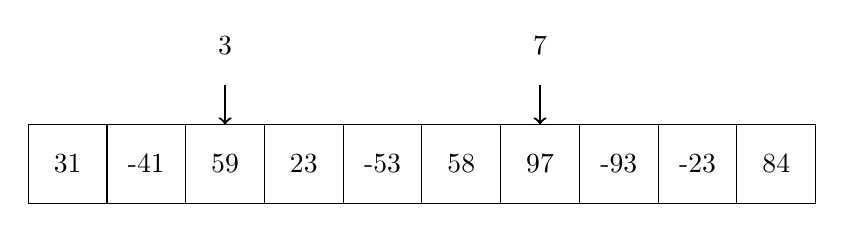
\begin{tikzpicture} \foreach \x [count=\i] in {31, -41, 59,
                    23, -53, 58, 97, -93, -23, 84} { \node[draw, minimum
                    size=1cm] at (\i,0) {\x}; } \draw[->, thick] (3,1) --
                    (3,0.5); \draw[->, thick] (7,1) -- (7,0.5); \node at
                (3,1.5) {3}; \node at (7,1.5) {7}; \end{tikzpicture}
            \end{center} Så returnerar den kubiska algoritmen svaret
            $X[3..7]$ och summan av den underarrayen är $187$. Så vad är
            det för fel på den? Jo, problemet är att den är långsam.
            Algoritmens yttre loop $(for~L~:=~1~to~N~do)$ körs $N$ gånger
            då $L$ är startindex på underarrayen och den måste söka
            \textbf{varje} möjlig underarray, och den mellersta loopen
            $(for~U~:=~L~to~N~do)$ där $U$ är slutindex på underarrayen och
            kan däför inte vara mindre än $L$, som körs högst $N$ gånger
            för varje körning av den yttre loopen. Till sist har vi
            ytterligare en loop, $(for~I~:=~L~to~U~do)$ där $I$ är index
            inom underarrayen och det är här som vi räknar summan av
            elementen i underarrayen, inom mellersta loopen som också körs
            högst $N$ gånger. Slutligen när vi multiplicerar stegen från
            vardera loop får vi en komplexitet på $O\left(N^3\right)$,
            därav namnet kubisk algoritm.
            %
            \section{Kvadratiska Algoritmer} Det finns två sätt att
            reducera komplexiteten till $O\left(N^2\right)$, liksom den
            kubiska algoritmen har dessa algoritmer fått namnet från sin
            komplexitet. Trots liknaden i komplexitet är utförningen
            väldigt olika. \label{kvadratisk} \subsection*{Den Första
            Kvadratiska Algoritmen} \label{sec:kvadratisk1} Här har man
            kunnat ta bort en av de nästlade looparna genom att använda sig
            av resultat från $X[L..U - 1]$ för att snabbare lösa $X[L..U]$:
            \begin{verbatim} MaxSoFar := 0.0 for L := 1 to N do Sum := 0.0
            for U := L to N do Sum := Sum + X[U] MaxSoFar := max(MaxSoFar,
            Sum) \end{verbatim} Om vi tar en noggrannare titt på hur
            algoritmen fungerar så ser vi att den yttre loopen räknar
            summan av de möjliga underarrayer $X[L..U]$ men märkväl att vi
            också memorerar summan för varje iteration för att tricket med
            den här algoritmen är att i den inre loopen tar vi helt enkelt
            uträkningen från $U - 1$ och adderar $X[U]$ vid $Sum := Sum +
            X[U]$ istället för att räkna summan av alla tal för varje $U$.
            %
            \subsection*{Den Andra Kvadratiska Algoritmen}
            \label{sec:kvadratisk2} Denna algoritm tänker om helt och
            börjar istället med att skapa en ny array som man kallar
            Cumulative Array eller Prefix Sum. Den nya arrayen sparar
            summan av nummer från början av den originala arrayen i varje
            steg $X[I]$ fram till det sista numret $X[N]$. \begin{verbatim}
            CumArray[0] := 0.0 for I := 1 to N do CumArray[I] :=
            CumArray[I-1] + X[I] MaxSoFar := 0.0 for L := 1 to N do for U
            := L to N do Sum := CumArray[U] - CumArray[L-1] MaxSoFar :=
            max(MaxSoFar, Sum) \end{verbatim} Första steget sätter
            $CumArray[0] := 0.0$ som fungerar som nollposition, sedan för
            varje $I$ beräknas $CumArray[I]$ genom att addera värdet $X[I]$
            till förra $CumArray[I - 1]$. Det låter säkert bekant och det
            är för att den förra algoritmen beräknade på samma sätt, men
            skillnaden här är att vi endast räknar på dem underarrayer där
            $L = 1$. En visualisering av en kort array som visar vilken
            summa index $2$ och $3$ skulle ha i $CumArray$: \begin{center}
                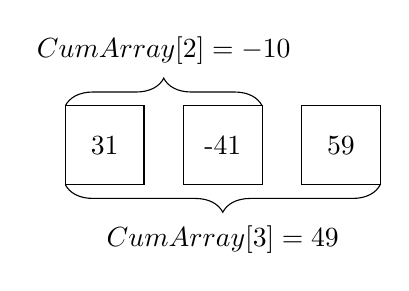
\begin{tikzpicture} \foreach \i [count=\n from 1] in {31,
                    -41, 59} { \node[draw, minimum size=1cm] at (1.5*\n,0)
                    {\i}; }
                    \draw[decorate,decoration={brace,amplitude=10pt}]
                    (1,0.5) -- (3.5,0.5)
                    node[midway,xshift=0.4cm,yshift=-0.4cm] {};
                    \draw[decorate,decoration={brace,amplitude=10pt}]
                    (5,-0.5) -- (1,-0.5)
                    node[midway,xshift=0.4cm,yshift=-0.4cm] {}; \node at
                    (2.25,1.2) {$CumArray[2] = -10$}; \node at (3,-1.2)
                {$CumArray[3] = 49$}; \end{tikzpicture} \end{center} Nu har
                vi sparat summorna i minnet och därefter kör en ny loop som
                är lik de första två men skiljer sig i inre loopen, här
                använder vi oss av summor vi har sparat i minnet och utför
                en enkel subtraktion av två olika summor från underarrayer
                vilket ger oss nya underarrayer där vi 'flyttar' på $L$,
                och sedanefter jämför den summan med den senaste största
                summan.
                %
                \section{Diskussion och slutsatser} \label{sec:disk} Vi har
                presenterat tre olika algoritmer som räknar den underarray
                med högst summa. Den kubiska algoritmen är enkel att förstå
                men ineffektiv för stora datamängder på grund av dess
                $O\left(N^3\right)$ komplexitet. De två kvadratiska
                algoritmerna förbättrar prestandan markant men på olika
                sätt och beroende på hur algoritmerna ska användas så
                finner man fördelar och nackdelar med båda vilket hjälper
                till att besluta vilken man vill använda. T.ex.~kan andra
                algoritmen som använder sig av $CumArray$ vara bra om man
                inte endast vill veta den högsta summan i en underarray
                utan flera olika. Eftersom den sparar i minnet skulle man
                få en konstant komplexitet $O\left(1\right)$, alltså endast
                1 steg, för varje underarray man frågar efter.
                %
                \begin{thebibliography}{99}
                        %
                    \bibitem{latexcompanion} Jon Bentley.
                        \textit{Programming pearls}.  Algorithm design
                        techniques, 27(9):865-866, 1984.
                        %
                \end{thebibliography}
            \end{document}
